\documentclass[11pt,a4paper,openright]{article}
\usepackage[spanish]{babel}
\usepackage{caption}
\usepackage{subcaption}
\usepackage{xcolor}
\usepackage{listings}
\usepackage{amsmath}
\usepackage{amsfonts}
\usepackage{amssymb}
\usepackage{float}
\usepackage{graphicx}
\usepackage{wrapfig}

\usepackage{vmargin}

\setpapersize{A4}
\setmargins{1.5cm}       % margen izquierdo
{1.5cm}                        % margen superior
{17.5cm}                      % anchura del texto
{23.42cm}                    % altura del texto
{8pt}                           % altura de los encabezados
{.5cm}                           % espacio entre el texto y los encabezados
{0pt}                             % altura del pie de página
{1.5cm} 
\lstset{literate=
  {á}{{\'a}}1 {é}{{\'e}}1 {í}{{\'i}}1 {ó}{{\'o}}1 {ú}{{\'u}}1
  {Á}{{\'A}}1 {É}{{\'E}}1 {Í}{{\'I}}1 {Ó}{{\'O}}1 {Ú}{{\'U}}1
  {à}{{\`a}}1 {è}{{\`e}}1 {ì}{{\`i}}1 {ò}{{\`o}}1 {ù}{{\`u}}1
  {À}{{\`A}}1 {È}{{\'E}}1 {Ì}{{\`I}}1 {Ò}{{\`O}}1 {Ù}{{\`U}}1
  {ä}{{\"a}}1 {ë}{{\"e}}1 {ï}{{\"i}}1 {ö}{{\"o}}1 {ü}{{\"u}}1
  {Ä}{{\"A}}1 {Ë}{{\"E}}1 {Ï}{{\"I}}1 {Ö}{{\"O}}1 {Ü}{{\"U}}1
  {â}{{\^a}}1 {ê}{{\^e}}1 {î}{{\^i}}1 {ô}{{\^o}}1 {û}{{\^u}}1
  {Â}{{\^A}}1 {Ê}{{\^E}}1 {Î}{{\^I}}1 {Ô}{{\^O}}1 {Û}{{\^U}}1
  {ã}{{\~a}}1 {ẽ}{{\~e}}1 {ĩ}{{\~i}}1 {õ}{{\~o}}1 {ũ}{{\~u}}1
  {Ã}{{\~A}}1 {Ẽ}{{\~E}}1 {Ĩ}{{\~I}}1 {Õ}{{\~O}}1 {Ũ}{{\~U}}1
  {œ}{{\oe}}1 {Œ}{{\OE}}1 {æ}{{\ae}}1 {Æ}{{\AE}}1 {ß}{{\ss}}1
  {ű}{{\H{u}}}1 {Ű}{{\H{U}}}1 {ő}{{\H{o}}}1 {Ő}{{\H{O}}}1
  {ç}{{\c c}}1 {Ç}{{\c C}}1 {ø}{{\o}}1 {å}{{\r a}}1 {Å}{{\r A}}1
  {€}{{\euro}}1 {£}{{\pounds}}1 {«}{{\guillemotleft}}1
  {»}{{\guillemotright}}1 {ñ}{{\~n}}1 {Ñ}{{\~N}}1 {¿}{{?`}}1 {¡}{{!`}}1 
}
\usepackage{listings}
\usepackage{xcolor}

\definecolor{codegreen}{rgb}{0,0.6,0}
\definecolor{codegray}{rgb}{0.5,0.5,0.5}
\definecolor{codepurple}{rgb}{0.58,0,0.82}
\definecolor{backcolour}{rgb}{0.95,0.95,0.92}

\lstdefinestyle{mystyle}{
    backgroundcolor=\color{backcolour},   
    commentstyle=\color{codegreen},
    keywordstyle=\color{magenta},
    numberstyle=\tiny\color{codegray},
    stringstyle=\color{codepurple},
    basicstyle=\ttfamily\footnotesize,
    breakatwhitespace=false,         
    breaklines=true,                 
    captionpos=b,                    
    keepspaces=true,                 
    numbers=left,                    
    numbersep=5pt,                  
    showspaces=false,                
    showstringspaces=false,
    showtabs=false,                  
    tabsize=2
}

\lstset{style=mystyle}

\usepackage{makeidx}
\usepackage{latexsym}
\title{Entrega 5 GCOM}
\author{Enrique Ernesto de Alvear Doñate}
\graphicspath{{C:/Users/Administrador/Pictures/}}
\begin{document}
\maketitle
\section{Introducción:}
Queremos comprobar como se deforma una esfera quitando el polo norte con una proyección. Para poder verlo mejor vamos a utilizar una curva contenida en la esfera. Usaremos la esfera unidad $\mathbb{S}^2$. Lo haremos de dos formas distintas:
\begin{enumerate}
\item[i)] Primero usaremos una proyección estereográfica con $\alpha=0.5$, y mostraremos como queda la esfera después de la proyección.
\item[ii)]Aquí utilizaremos una familia paramétrica para ver como se va deformando la esfera y mostraré el resultado con un gif.
\end{enumerate}
\section{Metodología:}
Primero vamos a coger una malla regular de puntos de la esfera con $\varphi \in [0,2\pi)$ y $\phi \in [0,\pi)$. Y para la curva voy a coger la curva de ecuaciones:
\begin{eqnarray*}
%\begin{equation}
x=cos^2(t)\\
y=sin(t)\\
z=cos(t)sin(t)
%\end{equation}
\end{eqnarray*}
La esfera que vamos a proyectar será esta:
\begin{figure}[H]
\centering
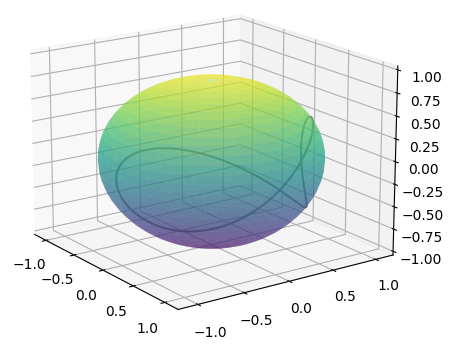
\includegraphics[scale=.75]{Esfera.png}
\end{figure}
\begin{enumerate}
\item[i)]Para hacer esto primero vamos a coger todos los puntos de la esfera y de la curva y proyectarlos utilizando la fórmula:
\begin{equation*}
x_i\prime=\frac{x_i}{(1-z)^\frac{1}{2}}
\end{equation*}

\item[ii)]En este apartado usaremos la familia paramétrica:\\
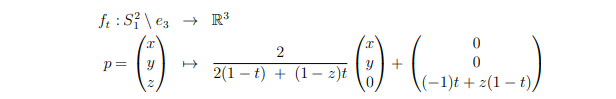
\includegraphics[scale=1.5]{famparam.png}\\
Para hacer el gif iremos variando el valor de t entre 0 y 1, y haremos para cada uno de esos valores la imagen de los puntos de la esfera respecto de la familia paramétrica.
\end{enumerate}
\section{Resultados:}
\begin{enumerate}


\item[i)]Como podemos ver en la gráfica siguiente:\\
\begin{figure}[H]
\centering
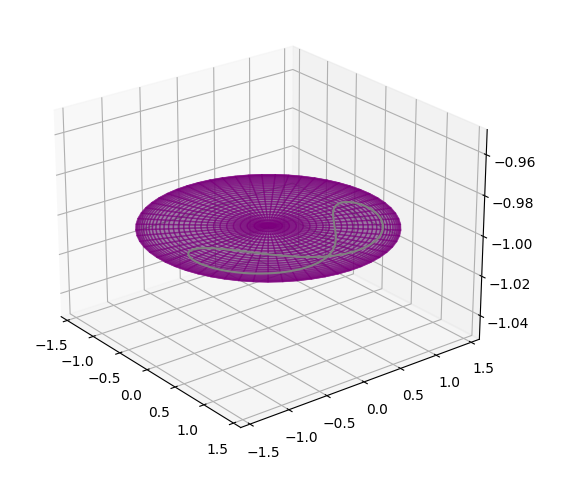
\includegraphics[scale=.85]{Proyeccion1.png}
\caption{Proyección estereográfica de la esfera y de la curva}
\end{figure}
\item[ii)] En el archivo .gif adjunto a este documento podemos ver la animación de nuestra familia paramétrica, a la cual hemos quitado el polo norte para que fuese bien todo.
\end{enumerate}
\newpage
\section{Anexo: código utilizado}
\lstinputlisting[language=Python]{Practica5EEAD.py}
\end{document}